\documentclass[a4paper]{article} 

\input{head}

\usepackage{float}
\usepackage[T1]{fontenc}
\usepackage{hyperref}
\usepackage{subcaption}

\begin{document}

\fancyhead[C]{}
\hrule \medskip
\begin{minipage}{0.295\textwidth} 
  \raggedright
  \scriptsize
  Michele Scomina \hfill\\   
  IN2000214\hfill\\
  mscomina@gmail.com\hfill\\
  michele.scomina@studenti.units.it
\end{minipage}
\begin{minipage}{0.4\textwidth} 
\centering 
\large 
\textbf{OpenMP and MPI - Mandelbrot Set}\\ 
\end{minipage}
\begin{minipage}{0.295\textwidth} 
\raggedleft
\today\hfill\\
\end{minipage}
\medskip\hrule 
\bigskip

\setlength{\parskip}{4pt}

\begin{abstract}
This is the report for Exercise 2. In this report we showcase the results of a hybrid MPI/OpenMP implementation of Exercise 2c, 
as described in the \href{https://github.com/Foundations-of-HPC/High-Performance-Computing-2023/tree/main/ASSIGNMENTS/exercise2}{GitHub repository}.
\end{abstract}

\section{Mandelbrot Set}
\subsection{Algorithm}
The Mandelbrot set algorithm maps each pixel $(x,y)$ to its corresponding point $c$ in the complex plane. For each point, it iteratively computes $z_{n+1}=z_n^2+c$ until either $|z_n|\geq2$ or the maximum number of iterations is reached. For each point, the iteration count at which the sequence escapes is stored in the corresponding pixel. If the maximum number of iterations is reached without escape, the pixel is assigned the value 0.

\begin{figure}[H]
    \centering
    
\includegraphics[width=0.7\textwidth]{mandelbrot.png}
    \caption{The Mandelbrot fractal.}
    \label{fig:mandelbrot}
\end{figure}


\subsection{Initial considerations}
The Mandelbrot set computation is trivially easy to parallelize: every pixel computed is assumed to be completely independent of the others. That makes the action of spreading the workload extremely easy among threads and processes alike.

However, there is an important consideration to make: \textbf{the Mandelbrot set's complexity is not evenly distributed} among the pixels, which means the implementation has to take care of a highly irregular computational workload. Naively partitioning the complex plane and assigning a fixed number of pixels to each thread or process can lead to significant load imbalance.


\newpage

\section{Benchmarking}
Before discussing the OpenMP/MPI implementations, it's important to define what kind of benchmark they will be tested against.
The weak and strong scaling of both OpenMP and MPI are tested on a computationally demanding region of the Mandelbrot set:

\begin{equation}
    z_{bl} = 0.35787121 + 0.1081397025i, z_{tr} = z_{bl} + (1+i)*10^{-8}, I_{max} = 3000
\end{equation}

\begin{figure}[H]
    \centering
    
\includegraphics[width=0.5\textwidth]{difficult_mandelbrot.png}
    \caption{Mandelbrot section used for benchmarking.}
    \label{fig:mandelbrot_benchmarking}
\end{figure}

Each configuration was executed 5 times across 4 THIN nodes of the ORFEO cluster, and the measured wall-clock execution times were averaged to reduce the impact of run-to-run variability. The benchmark has been run on the \texttt{/fast} partition for faster I/O operations.
\subsection{Scaling analysis}
The benchmark tests for two kinds of scaling: \textbf{strong} and \textbf{weak} scalability.

\begin{itemize}
\item \textbf{Strong scalability} describes how the execution time of a fixed-size problem changes as the number of computational resources is increased. In this specific case, the test consists in a \textbf{2048$\times$2048 region} of the computationally demanding Mandelbrot area.
\item \textbf{Weak scalability} describes how the execution time changes as both the problem size and the number of computational resources are increased proportionally, such that the amount of work assigned to each resource remains approximately constant. In this case, the baseline problem size is a \textbf{512$\times$512 region}. The side lengths of the region are \textbf{increased proportionally to the square root of the number of processes}, ensuring that the total number of pixels, and therefore the computational workload, grows approximately linearly with the number of processes. Ideally, the execution time should remain approximately constant as the number of processes increases.
\end{itemize}

\section{OpenMP}
\subsection{Implementation}
OpenMP is the most straightforward parallelization to implement, since OpenMP already provides dynamic scheduling through the \textbf{schedule(dynamic)} clause and it can be applied directly to the y, x loop over the pixels. Although dynamic scheduling introduces additional scheduling overhead, the improved load balancing significantly outweighs this cost for this workload.\\
To parallelize the code we wrap the y, x for loops with an \texttt{OMP PARALLEL FOR} directive with the following parameters:

\begin{figure}[H]
    \centering
    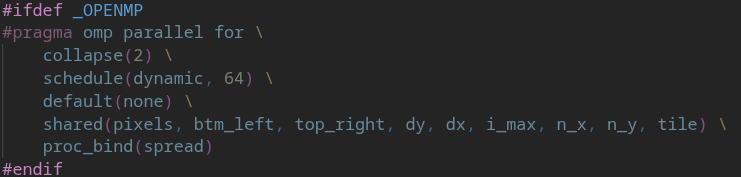
\includegraphics[width=0.7\textwidth]{openmp_code.png}
    \caption{OpenMP directive.}
    \label{fig:openmp_code}
\end{figure}

Several chunk sizes were evaluated experimentally. A chunk size of 64 provided the lowest average execution time among the tested configurations, representing a good trade-off between load balancing and scheduling overhead. Smaller chunks improve load balancing but increase scheduling overhead, while larger chunks reduce scheduling overhead at the cost of potentially greater load imbalance. The collapse(2) clause combines the two nested loops into a single iteration space, allowing OpenMP to distribute individual pixel computations more flexibly among threads.

\subsection{Scaling}

Both weak and strong OpenMP scaling show good scalability:

\begin{figure}[H]
    \centering

    \begin{subfigure}[b]{0.48\textwidth}
        \centering
        \includegraphics[width=\textwidth]{omp_weak.pdf}
        \caption{Weak OpenMP scaling.}
        \label{fig:omp_weak}
    \end{subfigure}
    \hfill
    \begin{subfigure}[b]{0.48\textwidth}
        \centering
        \includegraphics[width=\textwidth]{omp_strong.pdf}
        \caption{Strong OpenMP scaling.}
        \label{fig:omp_strong}
    \end{subfigure}

    \caption{Plots for OpenMP scaling averaged over 5 runs.}
    \label{fig:openmp_scaling}
\end{figure}

For strong scaling, increasing the number of threads from 2 to 24 gives a speedup of approximately 8 rather than the ideal factor of 12. This reduced scalability is likely due in part to the fixed problem size: as more threads are added, the amount of computation assigned to each thread decreases, while thread scheduling and synchronization overheads remain. At higher thread counts, these overheads therefore represent a larger fraction of the total execution time, limiting the achievable speedup.

In contrast, the weak-scaling results show that the workload remains sufficiently large as the number of threads increases. The execution time increases only slightly, from 1.22s to 1.29s, indicating that the additional computational work is effectively compensated for by the additional threads.

\newpage

\section{MPI}
\subsection{Implementation}
MPI requires more careful consideration than the OpenMP implementation because a simple static distribution of the image, for example using \texttt{MPI\_Scatter} followed by \texttt{MPI\_Reduce}, does not account for the irregular computational workload of the Mandelbrot set. Different regions of the complex plane can require significantly different numbers of iterations, so assigning a fixed number of pixels to each process can result in substantial load imbalance.\\

The approach we ended up using is a \textbf{master/worker} separation of processes:

\begin{itemize}
\item The \textbf{master process} is responsible for scheduling the computation and collecting the results from the workers. The image is divided into horizontal sections, referred to as \textit{tiles}, which are dynamically assigned to the workers.

\item The \textbf{worker processes} receive a tile from the master, perform the Mandelbrot computation for all pixels contained in that tile, and send the computed results back to the master. Once a worker finishes its computation, it is assigned another tile if there is still work available.

\item The number of tiles is set to \textbf{four times the number of worker processes}. This provides several tiles per worker, allowing the master to distribute the workload dynamically and compensate for the irregular computational cost of different regions of the Mandelbrot set. At the same time, the tiles are kept sufficiently large to avoid excessive communication and scheduling overhead.

\item This dynamic distribution helps prevent workers that finish computationally cheaper tiles from remaining idle while other workers are still processing more expensive regions. The choice of four tiles per worker therefore represents a compromise between fine-grained load balancing and the overhead introduced by communicating a large number of small tiles.

\end{itemize}

This approach therefore trades some communication and scheduling overhead for improved load balancing, which is particularly important for the irregular computational workload of the Mandelbrot set.

\subsection{Scaling}

Both weak and strong MPI scaling show good scalability as well:
\begin{figure}[H]
    \centering

    \begin{subfigure}[b]{0.48\textwidth}
        \centering
        \includegraphics[width=\textwidth]{mpi_weak.pdf}
        \caption{Weak MPI scaling.}
        \label{fig:mpi_weak}
    \end{subfigure}
    \hfill
    \begin{subfigure}[b]{0.48\textwidth}
        \centering
        \includegraphics[width=\textwidth]{mpi_strong.pdf}
        \caption{Strong MPI scaling.}
        \label{fig:mpi_strong}
    \end{subfigure}

    \caption{Plots for MPI scaling averaged over 5 runs.}
    \label{fig:mpi_scaling}
\end{figure}

For strong scaling, increasing the number of processes from 2 to 24 reduces the execution time from approximately 14s to 1.8s, corresponding to a speedup of approximately 8 rather than the ideal factor of 12. This is likely due to the communication and scheduling overhead introduced by the master/worker approach. As the number of processes increases, each worker performs less computation while the relative cost of distributing tiles and collecting results increases. Additionally, the processes were distributed across four different cluster nodes, introducing additional inter-node communication overhead.

The weak-scaling results show a larger increase in execution time, from 1.25s with 2 processes to 1.95s with 24 processes. A particularly noticeable spike occurs at 6 processes, which can be attributed to the workload requiring resources from an additional cluster node. This introduces additional inter-node communication and resource-management overhead, resulting in a temporary increase in execution time that is not directly representative of the general scaling trend. Beyond this point, the execution time remains relatively stable, although it gradually increases as the number of processes grows. Ideally, the execution time would remain constant as the problem size increases; the observed increase can be attributed to communication and scheduling overhead, which becomes more significant as the number of processes increases. Nevertheless, the execution time remains relatively stable compared to the increase in the total workload.

\section{Conclusions}
The results show that both the OpenMP and MPI implementations achieve good scalability for the Mandelbrot set computation. OpenMP provides good scaling on a single shared-memory system, while the MPI implementation is able to efficiently distribute the irregular workload across multiple processes and nodes. In both cases, the scaling is not ideal due to scheduling and communication overhead, which becomes more significant as the number of computational resources increases.

One possible improvement to the MPI implementation would be to allow the master process to perform computation when the number of processes is small. Currently, the master is dedicated to scheduling and communication, leaving one process unavailable for computation. Allowing it to also act as a worker could improve resource utilization, particularly for configurations with a small number of processes.
\end{document}